\appendix
\onecolumn
\section{Background on Riemannian Geometry}
\label{riemannian_geometry_appendix}
An $n$-dimensional manifold is a topological space that is equipped with a family of open sets $U_i$ which cover the space and a family of functions $\psi_i$ that are homeomorphisms between the $U_i$ and open subsets of $\mathbb{R}$.  The pairs $(U_i,\psi_i)$ are called \emph{charts}.  A crucial requirement is that if two open sets $U_i$ and $U_j$ intersect in a region, call it $U_{ij}$, then the composite map $\psi_i\circ \psi_j^{-1}$ restricted to $U_{ij}$ is infinitely differentiable. If $\mathcal{M}$ is an $n-$dimensional manifold then a chart, $\psi: U \to V$, on $\mathcal{M}$ maps an open subset $U$ to an open subset $V \subset \mathbb{R}^n$. Furthermore, the image of the point $p \in U$, denoted $\psi(p) : \mathbb{R}^n$ is termed the local coordinates of $p$ on the chart $\psi$. Examples of manifolds include $\mathbb{R}^n$, the Hypersphere $\mathbb{S}^n$, the Hyperboloid $\mathbb{H}^n$, a torus. In this paper we take an extrinsic view of the geometry, that is to say a manifold can be thought of as being embedded in a higher dimensional Euclidean space, ---i.e. $\mathcal{M}^n \subset \mathbb{R}^{n+1}$, and inherits the coordinate system of the ambient space. This is not how the subject is usually developed but for spaces of constant curvature one gets convenient formulas.

\xhdr{Tangent Spaces} Let $p \in \mathcal{M}$ be a point on an $n-$dimensional smooth manifold and let $\gamma(t) \to \mathcal{M}$ be a differentiable parametric curve with parameter $t \in [-\epsilon, \epsilon]$ passing through the point such that $\gamma(0) = p$. Since $\mathcal{M}$ is a smooth manifold we can trace the curve in local coordinates via a chart $\psi$ and the entire curve is given in local coordinates by $x = \psi \circ \gamma(t)$. The tangent vector to this curve at $p$ is then simply $v = (\psi \circ \gamma)'(0)$. Another interpretation of the tangent vector of $\gamma$ is by interpreting the point $p$ as a position vector and the tangent vector is then interpreted as the velocity vector at that point.\cut{Stated another way the tangent vector is a vector of partial derivatives for every coordinate.} Using this definition the set of all tangent vectors at $p$ is denoted as $\mathcal{T}_p{\mathcal{M}}$, and is called the tangent space at $p$. 

\xhdr{Riemannian Manifold}
A Riemannian metric tensor $g$ on a smooth manifold $\mathcal{M}$ is defined as a family of inner products such that at each point $p \in \mathcal{M}$ the inner product takes vectors from the tangent space at $p$, $g_p= \langle \cdot, \cdot \rangle_p: \mathcal{T}_p\mathcal{M} \times \mathcal{T}_p\mathcal{M} \to \mathbb{R}$. This means $g$ is defined for every point on $\mathcal{M}$ and varies smoothly. Locally, $g$ can be defined using the basis vectors of the tangent space $g_{ij}(p) = g(\frac{\partial}{\partial p_i}, \frac{\partial}{\partial p_j})$. In matrix form the Riemannian metric, $G(p)$, can be expressed as, $\forall u,v \in  \mathcal{T}_p\mathcal{M} \times \mathcal{T}_p\mathcal{M}, \langle u, v \rangle_p = g(p)(u,v) = u^T G(p) v$. A smooth manifold manifold $\mathcal{M}$ which is equipped with a Riemannian metric at every point $p \in \mathcal{M}$ is called a Riemannian manifold. Thus every Riemannian manifold is specified as the tuple $(\mathcal{M},g)$ which define the smooth manifold and its associated Riemannian metric tensor.

Armed with a Riemannian manifold we can now recover some conventional geometric insights such as the length of a parametric curve $\gamma$, the distance between two points on the manifold, local notion of angle, surface area and volume. We define the length of a curve, $L[\gamma] = \int_a^b g_{\gamma (t)} || \gamma '(t)|| dt$. This definition is very similar to the length of a curve on Euclidean spaces if we just observe that the Riemannian metric is $I_n$. Now turning to the distance between points $p$ and $q$ we can reason that it must be the smallest or distance minimizing parametric curve between the points which in the literature are known as \textit{geodesics}\footnote{Actually a geodesic is usually defined as a curve such that the tangent vector is parallel transported along it. It is then a theorem that it gives the shortest path.}. Stated another way: $d(p,q) = \inf \big\{ L[\gamma] \ | \gamma:[a,b] \to \mathcal{M}\big\}$ with ,  $\gamma(a)=p$ and $\gamma(b)=q$. A norm is induced on every tangent space by $g_p$ and is defined as $\mathcal{T}_p\mathcal{M}: || \cdot ||_p :\sqrt{\langle \cdot, \cdot \rangle_p}$. Finally, we can also define an infitisimal volume element on each tangent space and as a result measure $d\mathcal{M}(p) = \sqrt{|G(p)|} dp$, with $dp$ being the Lebesgue measure. 

\section{Background Normalizing Flows}
\label{normalizing_flow_appendix}
Given a parametrized density on $\mathbb{R}^n$ a \textit{normalizing flow} defines a sequence of invertible transformations to a more complex density over the same space via the change of variable formula for probability distributions \cite{rezende2015variational}. Starting from a sample from a base distribution, $z_0 \sim p(z)$, a mapping $f: \mathbb{R}^d \to \mathbb{R}^d$, with parameters $\theta$ that is both invertible and smooth, the log density of $z' = f(z_0)$ is defined as $\log p_{\theta}(z') = \log p(z_0) - \log \det \Big \lvert \frac{\partial f}{\partial z} \Big \rvert$.
\cut{
\begin{align}
    \log p_{\theta}(z') = \log p(z_0) - \log \det \Big \lvert \frac{\partial f}{\partial z} \Big \rvert.
    \label{flow_eqn_1}

\end{align}
}
Where, $p_{\theta}(z')$ is the probability of the transformed sample and $\partial f / \partial x$ is the Jacobian of $f$. To construct arbitrarily complex densities a chain of functions of the same form as $f$ can be defined and through successive application of change of density for each invertible transformation in the flow. Thus the final sample from a flow is then given by $z_j = f_j \circ f_{j-1} ... \circ f_1(z_0)$ and it's corresponding density can be determined simply by $\ln p_{\theta}(z_j) = \ln p(z_0) - \sum_{i=1}^j\ln \det \Big \lvert \frac{\partial f_i}{\partial z_{i-1}} \Big \rvert$. 
Of practical importance when designing normalizing flows is the cost associated with computed the log determinant of the Jacobian which is computationally expensive and can range anywhere from $O(n!)-O(n^3)$ for an arbitrary matrix and a chosen algorithm. However, through an appropriate choice of $f$ this computation cost can be brought down significantly. While there are many different choices for the transformation function, $f$, in this work we consider only RealNVP based flows as presented in \cite{dinh2016density} and \cite{rezende2015variational} due to their simplicity and expressive power in capturing complex data distributions.

\subsection{Variational Inference with Normalizing Flows}
One obvious use case for Normalizing Flows is in learning a more expressive often multi-modal posterior distribution needed in Variational Inference. Recall that a variational approximation is a lower bound to the data log-likelihood. Take for example amortized variational inference in a VAE like setting whereby the posterior $q_{\theta}$ is parameterized and is amenable to gradient based optimization. The overall objective with both encoder and decoder networks:
\begin{align}
    \log p(x) & = \log \int p(x|z)p(z) dz \\
              & \geq \mathbb{E}_{q_{\theta}(z|x)}[\log \frac{p(x,z)}{q_{\theta}(z|x)}] \ \ \ \  (\textnormal{Jensen's Inequality}) \\
              & = \mathbb{E}_{q_{\theta}(z|x)} [\log p(x|z)] + \mathbb{E}_{q_{\theta}(z|x)}\Big[\log \frac{p(z)}{q_{\theta}(z|x)}\Big] \\
              & = \mathbb{E}_{q_{\theta}(z|x)} [\log p(x|z)] - D_{KL}(q_{\theta}(z|x) || p(z)) \label{nn_vae_perspective}
\end{align}
The tightness of the Evidence Lower Bound (ELBO) also known as the negative free energy of the system, $-\mathcal{F}(x)$, is determined by the quality of the posterior approximation to the true posterior. Thus, one way to enrich the posterior approximation is by letting $q_{\theta}$ be a normalizing flow itself and the resultant latent code be the output of the transformation. If we denote $q_0(z_0)$ the probability of the latent code $z_0$ under the base distribution and $z_k$ as the latent code after $K$ flow layers we may rewrite the Free Energy as follows:

\begin{align}
    \mathcal{F}(x) &= \mathbb{E}_{q_{0}(z_0)}[\log q_k(z_j) - \log p(x,z_j)] \\
    &= \mathbb{E}_{q_{0}(z_0)}\Big[\log q_0(z_0) - \sum_{i=1}^j\ln \det \Big \lvert \frac{\partial f_i}{\partial z_{i-1}} \Big \rvert - \log p(x,z_i)\Big]\\
    &= D_{KL}(q_0(z_0)|| p(z_j)) - \mathbb{E}_{q_{0}(z_0)}\Big[\sum_{i=1}^j\ln \det \Big \lvert \frac{\partial f_i}{\partial z_{i-1}} \Big \rvert - \log p(x|z_i)\Big]
\end{align}
For convenience we may take $q_0 = \mathcal{N}(\mu, \sigma^2)$ which is a reparametrized gaussian density and $p(z) = \mathcal{N}(0, I)$ a standard normal. 

\subsection{Euclidean RealNVP}
\label{Euclidean_RealNVP_appendix}
Computing the Jacobian of functions with high-dimensional domain and codomain and computing the determinants of large matrices are in general computationally very expensive. Further complications can arise with the restriction to bijective functions make for difficult modelling of arbitrary distributions. A simple way to significantly reduce the computational burden is to design transformations such that the Jacobian matrix is triangular resulting in a determinant which is simply the product of the diagonal elements. In \cite{dinh2016density}, real valued non-volume preserving (RealNVP) transformations are introduced as simple bijections that can be stacked but yet retain the property of having the composition of transformations having a triangular determinant. To achieve this each bijection updates a part of the input vector using a function that is simple to invert,
but which depends on the remainder of the input vector in a complex way. Such transformations are denoted  as affine coupling layers. Formally, given a $D$ dimensional input $x$ and $d < D$, the output $y$ of an affine coupling layer follows the equations:
\begin{align}
    y_{1:d} & = x_{1:d} \\
    y_{d+1:D} & = x_{d+1:D} \odot \textnormal{exp}(s(x_{1:d})) + t(x_{1:d}).
\end{align}
Where, $s$ and $t$ are parameterized scale and translation functions. As the second part of the input depends on the first, it is easy to see that the Jacobian given by this transformation is lower triangular. Similarly, the inverse of this transformation is given by:
\begin{align}
     x_{1:d} & = y_{1:d} \\
    x_{d+1:D} & = (y_{d+1:D} - t(y_{1:d})\odot \textnormal{exp}(-s(y_{1:d})).
\end{align}
Note that the form of the inverse does not depend on calculating the inverses of either $s$ or $t$ allowing them to be complex functions themselves. Further note that with this simple bijection part of the input vector is never touched which can limit the expressiveness of the model. A simple remedy to this is to simply reverse the elements that undergo scale and translation transformations prior to the next coupling layer. Such an alternating pattern ensures that each dimension of the input vector depends in a complex way given a stack of couplings allowing for more expressive models. Finally, the Jacobian of this transformation is a lower triangular matrix,
\begin{equation} 
    \frac{\partial y}{\partial x} = \begin{bmatrix}
                                    \mathbb{I}_{d} & 0 \\
                                
                                   \frac{\partial y_{d+1:D}}{x^T_{1:d}} & \textnormal{diag}(\textnormal{exp}s(x_{1:d}))
                                    \end{bmatrix}.
\end{equation}

\section{Change of Variable for Tangent Coupling}
We now derive the change in volume formula associated with one $\mathcal{T}C$ layer. Without loss of generality we first define a binary mask which we use to partition the elements of a vector at $\mathcal{T}_{\textbf{o}}\mathbb{H}^n_K$ into two sets. Thus $b$ is defined as 
$$ 
b_j = 
\begin{cases}
1 &\textrm{if $j\leq d$}\\
0 &\textrm{otherwise},
\end{cases}
$$
Note that all $\mathcal{T}C$ layer operations exclude the first dimension which is always copied over by setting $b_0 = 1$ and ensures that the resulting sample always remains on $\mathcal{T}_{\textbf{o}}{\mathbb{H}^n_K}$. Utilizing $b$ we may rewrite Equation \ref{eq:tangent_coupling} as,

\label{tangent_coupling_proof_appendix}
\begin{equation}
    \textbf{y} =  \textnormal{exp}^K_{\textbf{o}}\big(b \odot \tilde{x} + (1 - b)\odot(\tilde{x} \odot \sigma(s(b \odot \tilde{x})) + t(b \odot \tilde{x}))\big),
\end{equation}
where $\tilde{x} = \log^K_{\textbf{o}}(x)$ is a point on the tangent space at $\textbf{o}$. Similar to the Euclidean RealNVP, we wish to calculate the jacobian determinant of this overall transformation. We do so by first observing that the overall transformation is a valid composition of functions: $y := \textnormal{exp}^K_{\textbf{o}} \circ f\circ \log^K_{\textbf{o}}(\textbf{x})$, where $z = f(\tilde{x})$ is the flow in tangent space. Utilizing the chain rule and the identity that the determinant of a product is the product of the determinants of its constituents we may decompose the jacobian determinant as,

\begin{equation}
    \textnormal{det}\Big (\frac{\partial \textbf{y}}{\partial \textbf{x}}\Big) =  \textnormal{det}\Big (\frac{\partial \textnormal{exp}^K_{\textbf{o}}(z)}{\partial z}\Big) \cdot \textnormal{det}\Big (\frac{\partial f(\tilde{x})}{\partial \tilde{x}}\Big) \cdot  \textnormal{det}\Big (\frac{\partial \log^K_{\textbf{o}}(\textbf{x})}{\partial \textbf{x}}\Big)
    \label{jac_det_tangent_flow_1}.
\end{equation}
Tackling each term on RHS of Eq. \ref{jac_det_tangent_flow_1} individually, $ \textnormal{det}\Big (\frac{\partial \textnormal{exp}^K_{\textbf{o}}(z)}{\partial z}\Big) = \Big(\frac{R\sinh(\frac{||z||_{\mathcal{L}}}{R})}{||z||_{\mathcal{L}}}\Big)^{n-1}$ as derived in \cite{nagano2019wrapped}. As the logarithmic map is the inverse of the exponential map the jacobian determinant is also the inverse ---i.e.  $\textnormal{det}\Big (\frac{\partial \log^K_{\textbf{o}}(\textbf{x})}{\partial \textbf{x}}\Big) = \Big(\frac{\sinh(||\log^K_{\textbf{o}}(\textbf{x})||_{\mathcal{L}})}{||\log^K_{\textbf{o}}(\textbf{x})||_{\mathcal{L}}}\Big)^{1-n}$. For the middle term in Eq. \ref{jac_det_tangent_flow_1} we proceed by selecting the standard basis $\{e_1, e_2, ... e_n\}$ which is an orthonormal basis  with respect to the Lorentz inner product. The directional derivative with respect to a basis element $e_j$ is computed as follows:

\begin{align*}
    \textnormal{d}f(\tilde{x}) &= \frac{\partial}{\partial \epsilon} \Big |_{\epsilon=0} f(\tilde{x} + \epsilon e_j)\\
    & = \frac{\partial}{\partial \epsilon} \Big |_{\epsilon=0} \{b \odot (\tilde{x} + \epsilon e_j) + (1 - b)\odot((\tilde{x} + \epsilon e_j) \odot \sigma(s(b \odot (\tilde{x} + \epsilon e_j))) + t(b \odot (\tilde{x} + \epsilon e_j)))\} \\
    &= b \odot  e_j + \frac{\partial}{\partial \epsilon} \Big |_{\epsilon=0}\{ (1 - b)\odot((\tilde{x} + \epsilon e_j) \odot \sigma(s(b \odot (\tilde{x} + \epsilon e_j))) + t(b \odot (\tilde{x} + \epsilon e_j)))\} \\
\end{align*}
As $b \in [0,1]^n$ is a binary mask, it is easy to see that if $b_j =1$ then only the first term on the RHS remains and the directional derivative with respect to $e_j$ is simply the basis vector itself. Conversely, if $b_j =0$ then the first term goes to zero and we are left with the second term,

\begin{align*}
    \textnormal{d}f(\tilde{x}) &= \frac{\partial}{\partial \epsilon} \Big |_{\epsilon=0}\{ (1 - b)\odot((\tilde{x} + \epsilon e_j) \odot \sigma(s(b \odot (\tilde{x} + \epsilon e_j))) + t(b \odot (\tilde{x} + \epsilon e_j)))\} \\
    &=  \frac{\partial}{\partial \epsilon} \Big |_{\epsilon=0}\{ (1 - b)\odot((\tilde{x} + \epsilon e_j) \odot \sigma(s(b \odot \tilde{x})) + t(b \odot \tilde{x}))\} \\
    &= e_j \odot \sigma(s(b \odot \tilde{x})).
\end{align*}
Where in the second line we've used the fact $b \odot \epsilon e_j = 0$. All together, the directional derivatives computed using our chosen basis elements are,

\begin{equation*}
    \textnormal{d}f(\tilde{x}) = (e_1, e_2, \dots e_d, e_{d+1}\odot \sigma(s(b \odot \tilde{x})), \dots e_{D}\odot \sigma(s(b \odot \tilde{x}))).
\end{equation*}
The volume factor given by this linear map is $\textnormal{det}( \textnormal{d}f(\tilde{x})) = \sqrt{G^TG}$, where $G$ is the matrix of all directional derivatives. As the basis elements are orthogonal all non-diagonal entries of $G^TG$ go to zero and the determinant is the product of the Lorentz norms of each component. As $||e_j||_{\mathcal{L}} =1$ and $||e_{j}\odot \sigma(s(b \odot \tilde{x}))||_{\mathcal{L}} = ||e_{j}\odot \sigma(s(b \odot \tilde{x}))||_2$ for $\mathcal{T}_{\mathbf{o}}H^n_K$ the overall determinant is then $\textnormal{d}f(\tilde{x}) = \textnormal{diag} \ \sigma(s(b \odot \tilde{x}))$. Finally, the full log jacobian determinant of a $\mathcal{T}C$ layer is given by,

\begin{equation}
    \log \textnormal{det}\Big (\frac{\partial \textbf{y}}{\partial \textbf{x}}\Big) = \Big(\frac{R\sinh(\frac{||z||_{\mathcal{L}}}{R})}{||z||_{\mathcal{L}}}\Big)^{n-1} + \sum_{i=d+1}^n\sigma(s(\tilde{x}_1))_i 
      + \Big(\frac{R\sinh(\frac{||\log^K_{\textbf{o}}(\textbf{x})||_{\mathcal{L}}}{R})}{||\log^K_{\textbf{o}}(\textbf{x})||_{\mathcal{L}}}\Big)^{1-n}
\end{equation}

Thus the overall computational cost is only slightly larger than the regular Euclidean RealNVP, $\mathcal{O}(n)$.

\section{Change of Variable for Wrapped Hyperbolic Coupling}
\label{wrapped_coupling_proof_appendix}
We consider the following function $f : \mathbb{H}^n_K \rightarrow \mathbb{H}^n_K$, which we use to define a normalizing flow in $n$-dimensional hyperbolic space (represented via the Lorentz model): 
\begin{equation}\label{eq:mainflow}
    f(\mb{x}) = \textnormal{exp}^K_{\textbf{o}}\left( b \odot \tilde{
    x} + (1-b) \odot \log^K_{\textbf{o}}\Big( \textnormal{exp}^K_{t(b \odot \tilde{x})}\big(\textnormal{PT}^K_{\textbf{o}\to t(b \odot \tilde{x}) }((1-b) \odot \tilde{x} \odot \sigma(s(b \odot \tilde{x})))\big)\Big) \right),
\end{equation}

where $\tilde{x} = \log_\mb{o}(\mb{x}) \in \mc{T}_\mb{o}\mbb{H}^n_K$ is the projection of $\mb{x} \in \mbb{H}^n_K$ to the tangent space at the origin, i.e, $\mc{T}_\mb{o}\mbb{H}^n_K$. As in $\mathcal{T}C$ we again utilize a binary mask $b$ so that
$$ 
b_j = 
\begin{cases}
1 &\textrm{if $j\leq d$}\\
0 &\textrm{otherwise},
\end{cases}
$$
where $0 < d < n$.
In Equation \eqref{eq:mainflow} the function $s : \mc{T}_o\mbb{H}^d_K \rightarrow \mc{T}_o\mbb{H}^{n-d}_K$ is an arbitrary function on the tangent space at the origin and $\sigma$ denotes the logistic function.
The function $t : \mc{T}_o\mbb{H}^d_K \rightarrow \mbb{H}^*_K \subset {H}^n_K$ is a map from the tangent space at the origin to a subset of hyperbolic space defined by the set of points satisfying the condition that $\mb{v}_i = 0, \forall i=2...d, \mb{v}_i \in \mbb{H}^n_K$ (under their representation in the Lorentz model).

Our goal is to derive the Jacobian determinant of $f$, i.e., 
\begin{equation}
    \left|\textrm{det}\left(\frac{\partial f(\mb{x})}{\partial \mb{x}}\right)\right|,
\end{equation}
%where $\frac{\partial f(\mb{x})}{\partial \mb{x}} : \mc{T}_\mb{x}\mbb{H}^n_K \rightarrow \mc{T}_{f(\mb{x})}\mbb{H}^n_K$ is Jacobian of $f$.
To do so, we will use the following facts without proof or justification:
\begin{itemize}
    \item 
    \textbf{Fact 1: }The chain rule for determinants, i.e., the fact that
    \begin{equation}
        \left|\textrm{det}\left(\frac{\partial f(\mb{x})}{\partial \mb{x}}\right)\right| =  \left|\textrm{det}\left(\frac{\partial f(\mb{x})}{\partial \mb{v}}\right)\right| \left|\textrm{det}\left(\frac{\partial \mb{v}}{\partial \mb{x}}\right)\right|,
    \end{equation}
    where $\mb{v}$ is introduced via a valid change of variables. 
    \item 
    \textbf{Fact 2: } The Jacobian determinant for the exponential map $\exp^K_\mb{u}(z) = \mc{T}_{u}\mbb{H}^n_K \rightarrow \mbb{H}^n_K$ is given by
    \begin{equation}
        \left|\textrm{det}(\exp^K_\mb{u}(z))\right| =
        \left(\frac{R\sinh(\frac{||z||_{\mathcal{L}}}{R})}{||z||_{\mathcal{L}}}\right)^{n-1}
    \end{equation}
        \item 
    \textbf{Fact 3: } The Jacobian determinant for the logarithmic map $\log^K_\mb{u}(\mb{v}) = \mbb{H}^n_K \rightarrow \mc{T}_u\mbb{H}^n_K$ is given by
    \begin{equation}
        \left|\textrm{det}(\log^K_\mb{u}(\mb{v})\right| =
        \left(\frac{R\sinh(\frac{||\log^K_{\textbf{o}}(\textbf{v})||_{\mathcal{L}}}{R})}{||\log^K_{\textbf{o}}(\textbf{v})||_{\mathcal{L}}}\right)^{1-n}
    \end{equation}
    \item
     \textbf{Fact 4: } The Jacobian determinant for parallel transport $\textnormal{PT}^K_{\mb{u} \rightarrow \mb{t}}(v) = \mc{T}_\mb{u}\mbb{H}^n_K \rightarrow \mc{T}_t\mbb{H}^n_K$ is given by
    \begin{equation}
        \left|\textrm{det}\left(\textnormal{PT}^K_{\mb{u} \rightarrow \mb{t}}(v)\right)\right| = 1.
    \end{equation}
\end{itemize}
Fact 2 and Fact 4 are proven in \citet{nagano2019wrapped} ``A Wrapped Normal Distribution on Hyperbolic Space for Gradient-Based Learning'' for $K=-1$ and rederived for general $K$ in \citet{skopek2019mixed}. Fact 3 follows from the fact that the determinant of the inverse of a function is the inverse of that function's determinant. 
We will use similar arguments to obtain our determinant as were used in \citet{nagano2019wrapped}, and we refer the reader to Appendix A.3 in their work for background. 

Our main claim is as follows
\begin{prop}
The Jacobian determinant of the function $\tilde{f}^{\mathcal{W}\mathbb{H}C}$ in \eqref{wrapped_hyperboloid_coupling_eqn} is:
\begin{multline}
  \left|\textnormal{det}\left(\frac{\partial\mb{y}}{\partial \mb{x}}\right)\right| = \prod_{i=d+1}^n\sigma(s(\tilde{x}_1))_i \times \Big(\frac{R \sinh(\frac{||q||_{\mathcal{L}}}{R})}{||q||_{\mathcal{L}}}\Big)^{l}
  \times \Big(\frac{R\sinh(\frac{||\log_{\textbf{o}}^K(\hat{\textbf{q}})||_{\mathcal{L}}}{R})}{||\log_{\textbf{o}}^K(q)||_{\mathcal{L}}}\Big)^{-l} \ \times  \Big(\frac{R\sinh(\frac{||\tilde{z}||_{\mathcal{L}}}{R})}{||\tilde{z}||_{\mathcal{L}}}\Big)^{n-1}
 \  \\ \times \Big(\frac{R\sinh(\frac{||\log_{\textbf{o}}^K(\textbf{x})||_{\mathcal{L}}}{R})}{||\log_{\textbf{o}}^K(\textbf{x})||_{\mathcal{L}}}\Big)^{1-n},
\end{multline}
where 
$$
z =  b \odot \tilde{
    x} + \log^K_{\textbf{o}}\Big( \textnormal{exp}^K_{t(b \odot \tilde{x})}\big(\textnormal{PT}^K_{\textbf{o}\to t(b \odot \tilde{x}) }((1-b) \odot \tilde{x} \odot \sigma(s(b \odot \tilde{x})))\big)\Big)
$$
the argument to the parallel transport $q$ is,
$$
 q = \textnormal{PT}^K_{\textbf{o}\to t(b \odot \tilde{x}) }((1-b) \odot \tilde{x} \odot \sigma(s(b \odot \tilde{x}))). 
$$
and
$$
\hat{\textbf{q}} = \textnormal{exp}_{\textbf{t}}^K(q)
$$
\end{prop}
\begin{proof}
We first note that 
\begin{equation}
\left|\textnormal{det}\left(\frac{\partial f(\mb{x})}{\partial \mb{x}}\right)\right| = \left|\textrm{det}\left(\frac{\partial f(\mb{x})}{\partial z}\right)\right| \times \left|\textrm{det}\left(\frac{\partial z}{\partial \tilde{x}}\right)\right| \times \left|\textrm{det}\left(\frac{\partial \tilde{x}}{\partial \mb{x}}\right)\right| 
\end{equation}
by the chain rule (recalling that $\tilde{x} = \log_\mb{o}(\mb{x})$).
Now, we have that 
\begin{equation}
\left|\textrm{det}\left(\frac{\partial f(\mb{x})}{\partial z}\right)\right| =
\Big(\frac{R\sinh(\frac{||z||_{\mathcal{L}}}{R})}{||z||_{\mathcal{L}}}\Big)^{n-1}
\end{equation}
by Fact 2.
And, 
\begin{equation}
\left|\textrm{det}\left(\frac{\partial \tilde{x}}{\partial \mb{x}}\right)\right| =
\Big(\frac{R\sinh(\frac{||\log^K_{\textbf{o}}(\textbf{x})||_{\mathcal{L}}}{R})}{||\log^K_{\textbf{o}}(\textbf{x})||_{\mathcal{L}}}\Big)^{1-n}
\end{equation}
by Fact 3.
Thus, we are left with the term
$$
\left|\textrm{det}\left(\frac{\partial z}{\partial \tilde{x}}\right)\right|.
$$
To evaluate this term, we rely on the following Lemma:

\begin{lemma}
Let $h : \mc{T}_\mb{o}\mbb{H}^n_K \rightarrow \mc{T}_\mb{o}\mbb{H}^n_K$ be a function from the tangent space at the origin to the tangent space at the origin defined as:
\begin{equation}\label{eq:g}
h(\tilde{x}) = z = b \odot \tilde{
    x} + \log^K_{\textbf{o}}\Big( \textnormal{exp}^K_{t(b \odot \tilde{x})}\big(\textnormal{PT}^K_{\textbf{o}\to t(b \odot \tilde{x}) }((1-b) \odot \tilde{x} \odot \sigma(s(b \odot \tilde{x})))\big)\Big).
\end{equation}
Now, define a function $h^* : \mc{T}_\mb{o}\mbb{H}^{n-d}_K \rightarrow \mc{T}_\mb{o}\mbb{H}^{n-d}_K$ which acts on the subspace of $\mc{T}_\mb{o}\mbb{H}^{n-d}_K$ corresponding to the standard basis elements $e_{d+1}, ..., e_n$ as
\begin{equation}\label{eq:gstar}
h^*(\tilde{x}_{d+1:n}) =   \log^K_{\mb{o}_{d+1:n}}\Big( \textnormal{exp}^K_{t_{d+1:n}}\big(\textnormal{PT}^K_{\mb{o}_{d+1:n} \to t_{d+1:n}}( \tilde{x}_{d+1:n} \odot \sigma(s))\big)\Big),
\end{equation}
where $\tilde{x}_{d+1:n}$ denotes the portion of the vector $\tilde{x}$ corresponding to the standard basis elements $e_{d+1}, ..., e_n$ and $s$ and $t$ are constants (which depend on $\tilde{x}_{2:d}$).
In \eqref{eq:gstar}, we use $\mb{o}_{d+1:n} \in \mbb{H}^{n-d}_K$ to denote the vector corresponding to only the dimensions $d+1, ..., n$ and similarily for $t_{d+1:n}$.
Then we have that
\begin{equation}
    \left|\textnormal{det}\left(\frac{\partial z}{\partial \tilde{x}}\right)\right| =    \left|\textnormal{det}\left(\frac{\partial h^*(\tilde{x}_{d+1:n})}{\partial \tilde{x}_{d+1:n})}\right)\right|.
\end{equation}
\end{lemma}
\begin{proof}
First note that by design we have that 
\begin{equation}
    [0,0..,0] \oplus h^*(\tilde{x}_{d+1:n}) = \log^K_{\textbf{o}}\Big( \textnormal{exp}^K_{t(b \odot \tilde{x})}\big(\textnormal{PT}^K_{\textbf{o}\to t(b \odot \tilde{x}) }((1-b) \odot \tilde{x} \odot \sigma(s(b \odot \tilde{x})))\big)\Big),
\end{equation}
i.e., the output of $h^*$ is equal to right hand side of Equation \eqref{eq:g} after prepending/concatenating 0s to the output of $h^*$. 

Now, we can evaluate 
$$
\left|\textrm{det}\left(\frac{\partial z}{\partial \tilde{x}}\right)\right|
$$
by examining the directional derivative with respect to a set of basis elements of $\mc{T}_\mb{o}\mbb{H}^{n}_K$.
Now, given that this is the tangent space at the origin, we know that the standard (i.e., Euclidean) basis elements $e_2, ..., e_n$ form a valid basis for this subspace, since they are orthogonal under the Lorentz normal and orthogonal to the origin itself. 
Now, we can note first that
\begin{equation}
    D_{e_i}h(\tilde{x}) = e_i, \forall i=2...d.
\end{equation}
In other words, the directional derivative for the first $d$ basis elements is the simply the basis elements themselves. This can be verified by taking the definition of the directional derivative:
\begin{equation}
     D_{e_i}h(\tilde{x})  = \frac{\partial}{\partial \epsilon}\Big|_{\epsilon = 0}h(\tilde{x} + \epsilon e_i)
\end{equation}
and noting that the 
$$
\log^K_{\textbf{o}}\Big( \textnormal{exp}^K_{t(b \odot \tilde{x})}\big(\textnormal{PT}^K_{\textbf{o}\to t(b \odot \tilde{x}) }((1-b) \odot \tilde{x} \odot \sigma(s(b \odot \tilde{x})))\big)\Big)
$$
term must equal zero since $(1-b)\odot e_i = 0, \forall i = 2, ..., d$ by design. 
Now, for the basis elements $e_i$ with $i>d$ we have that
\begin{equation}
     D_{e_i}h(\tilde{x}) \perp e_j, \forall i=d+1, ..., n, j=2...,d.
\end{equation}
This holds because 
\begin{align}
D_{e_i}h(\tilde{x})  &= \frac{\partial}{\partial \epsilon}\Big|_{\epsilon = 0}h(\tilde{x} + \epsilon e_i) \\
 &= \frac{\partial}{\partial \epsilon}\Big|_{\epsilon = 0}    \log^K_{\textbf{o}}\Big( \textnormal{exp}^K_{t(b \odot \tilde{x})}\big(\textnormal{PT}^K_{\textbf{o}\to t(b \odot \tilde{x}) }((1-b) \odot \tilde{x} \odot \sigma(s(b \odot \tilde{x})))\big)\Big) 
\end{align}
since $b \odot e_i = 0, \forall i = d+1, ..., n$ by design and because
\begin{equation}
   \log^K_{\textbf{o}}\Big( \textnormal{exp}^K_{t(b \odot \tilde{x})}\big(\textnormal{PT}^K_{\textbf{o}\to t(b \odot \tilde{x}) }((1-b) \odot \tilde{x} \odot \sigma(s(b \odot \tilde{x})))\big)\Big) \perp e_j, \forall \tilde{x} \in \mc{T}_\mb{o}\mbb{H}^n_K, \forall  j=2...,d.
\end{equation}
due to the $(1-b)$ term inside the parallel transport and by our design of the function $t$. 
Together, these facts give that the Jacobian matrix for $h$ (under the basis $e_2, ..., e_n$) has the following block form:
\begin{equation}
   \left(\frac{\partial z}{\partial \tilde{x}}\right) = \left[\begin{BMAT}{cc}{cc}
    I & \mb{0} \\
    A & \frac{\partial h^*(\tilde{x}_{d+1:n})}{\partial \tilde{x}_{d+1:n})}
    \end{BMAT}\right]
\end{equation}
and by the properties of determinants of block matrices we have that
\begin{equation}
    \left|\textnormal{det}\left(\frac{\partial z}{\partial \tilde{x}}\right)\right| =    \left|\textnormal{det}\left(\frac{\partial h^*(\tilde{x}_{d+1:n})}{\partial \tilde{x}_{d+1:n})}\right)\right|
\end{equation}
\end{proof}
Given Lemma 1, all that remains is to evaluate 
\begin{equation}
    \left|\textnormal{det}\left(\frac{\partial h^*(\tilde{x}_{d+1:n})}{\partial \tilde{x}_{d+1:n})}\right)\right|.
\end{equation}
This can again be done by the chain rule, where we use Facts 2-4 to compute the determinant for exponential map, logarithmic map, and parallel transport.
Finally, the Jacobian determinant for the term
\begin{equation}
    \tilde{x} \odot \sigma(s(b \odot \tilde{x})))
\end{equation}
can easily be computed as $\prod_{j=d+1}^n\sigma(s(b \odot \tilde{x}))_j$ since the standard Euclidean basis is a basis for the tangent space at the origin as shown in Appendix \ref{Euclidean_RealNVP_appendix}.
\end{proof}

\cut{

\section{Decoders}
\noindent
\textbf{Issue:} Our VGAE models are trained using a cross-entropy loss over the predictions
\begin{equation}
    \hat{P}(A[i,j] = 1 | \Theta),
\end{equation}
where $\Theta$ is our encoder/decoder model parameters. However, many of our decoders are not giving proper probabilities, 
for example taking a sigmoid of distances between node latents
\begin{equation}
    \hat{P}(A[i,j] = 1 | \Theta) = \sigma(-d(\mb{z}_i, \mb{z}_j))
\end{equation}
is improper since $\sigma(-d(\mb{z}_i, \mb{z}_j)) \in [0,0.5]$ and is not surjective onto $[0,1]$. (The root cause is the fact that $d(\mb{z}_i, \mb{z}_j) \geq 0$.)
{\bf Note that this is an issue at both training and inference, as our cross-entropy loss during training will also struggle to learn when using improper probability inputs.}


Note that the dot-product decoder does not have this problem because 
\begin{equation}
  \hat{P}(A[i,j] = 1 | \Theta) = \sigma(\mb{z}_i^\top \mb{z}_j) 
\end{equation}
is surjective on $[0,1]$ since $\mb{z}_i^\top \mb{z}_j\in [-\inf, \inf]$.
{\bf However, we want to use a distance-based decoder, because that allows us to leverage the structure of the hyperbolic space in the most proper/elegant/intuitive way.}\\

\noindent
\textbf{Direct Solution} We use a well-defined softmax. The most direct solution to give proper probabilties for edges within a single graph based on distances would be:
\begin{equation}
    \hat{P}(A[i,j] = 1 | \Theta) = \sigma(p)\times\frac{\exp(d(\mb{z}_i, \mb{z}_j))}{\sum_{k=1}^{n}\sum_{l=l+1}^{n}\exp(d(\mb{z}_k, \mb{z}_l))} 
\end{equation}
where $p \in \mathbb{R}$ is a learnable parameter that controls the density of the graph.  
Note that here we are normalizing over all possible edges in the graph. 
Thus, a pair of nodes that are close together {\em relative to the average pair of nodes in the graph}, will tend to be connected. 
The $\sigma(p)$ term controls the density of the graph. 
{\bf This equation would be perfect if we were only learning a model over a single graph... However, if we are training over a distribution of multiple graphs that might have different numbers of nodes then the probabilities will all be lower in larger graphs, which is no good.}
In particular, if all the nodes are equidistant then we will get lower probabilities for a graph with more nodes...
A natural way to fix this is as follows:
\begin{equation}
    \hat{P}^{\textrm{fixed}}(A[i,j] = 1 | \Theta) = \sigma(p)\times\frac{\exp(d(\mb{z}_i, \mb{z}_j))}{\sum_{k=1}^{n}\sum_{l=l+1}^{n}\exp(d(\mb{z}_k, \mb{z}_l))} \times \left(\max_{i',j'}\left\{\frac{\exp(d(\mb{z}_{i'}, \mb{z}_{j'}))}{\sum_{k=1}^{n}\sum_{l=l+1}^{n}\exp(d(\mb{z}_k, \mb{z}_l))}\right\}\right)^{-1}
\end{equation}
That is, we normalize the softmax score by the inverse of the maximum softmax value for a graph.
This ensures that the decoder simplifies to the Erdos-Renyi model (with edge probability $\sigma(p)$) when all pairwise distances are equal (in expectation), regardless of how many nodes are in the graph.
Note that the $\sigma(p)$ term is important since it is what allows the model to learn the density of the graph. 



}

\section{Model Architectures and Hyperparameters}
\label{model_arch_and_hyperparams}
In this section we provide more details regarding model architectures and hyperparameters for each experiment in \ref{experiments}. For all hyperbolic models we used a curvature warmup for $10$ epochs which aids in numerical stability \citet{skopek2019mixed}. Specifically, we set $R=11$ and linearly decrease to $R=2$ every epoch after which it is treated as a learnable parameter. 

\xhdr{Structured Density Estimation}
For all VAE models our encoder consists of three linear layers. The first layer maps the input to a hidden space and the other two layers are used to paramaterize the mean and variance of the prior distribution and map samples to the latent space. The decoder for these models is simply a small MLP that consists of two linear layers that map the latent space to the hidden space and then finally back to the observation space. One important distinction between Euclidean models and hyperbolic models is that we use aFor BDP the hidden dim size is $200$ while for MNIST we use $600$ and the latent space is varied as shown in Tables \ref{table:bdp_table} and \ref{table:mnist_table}. All flow models used in this setting consist of $2$ linear layers each of size $128$. Between each layer in either the encoder and decoder we use the LeakyRelu \cite{xu2015empirical} activation function while tanh is used between flow layers. Lastly, we train all models for $80$ epochs with the Adam optimizer with default setting \cite{kingma2014adam}.

\xhdr{Graph Reconstruction}
For graph reconstruction task we use the VGAE model as a base \cite{kipf2016variational} which also uses three linear layers of size $16$ as the encoder in the VAE model. The decoder however is parameter less and is simply an inner product either in Euclidean space or in $\mathcal{T}_{\textbf{o}}\mathbb{H}^n_K$ for Hyperbolic models. As the reconstruction objective contains $N^2$ terms we rescale the $\mathbb{D}_{KL}$ penalty by a factor of $1/N$ such that each of the losses are on the same scale. This can be understood as a $\beta-$VAE like model where $\beta = 1/N$. Like the structured density estimation setting all our flow models consist of two linear layers of size $128$ with a tanh nonlinearity. Finally, we train the each model for $3000$ epochs using the Adam optimizer \cite{kingma2014adam}. 

\xhdr{Graph Generation}
For the graph generation task we adapt the training setup from \cite{liu2019graph} in that we pretrain a graph autoencoder for $100$ epochs to generate node latents. Empirically, we found that using a VGAE model for hyperbolic space worked better than a vanilla a GAE model. Furthermore, instead of using simple linear layers for the encoder we use GAT \cite{velivckovic2017graph} layer of size $32$, which has access to the adjacency matrix. We use LeakyReLU for our encoder non-linearity while tanh is used for all flow models. Unlike GRevNets that use node features sampled from $\mathcal{N}(0,I)$ we find that it is necessary to provide the actual adjacency matrix otherwise training did not succeed. Our decoder defines edge probabilities as $p(A_{u,v}=1|z_u,z_v) = \sigma((-d_{\mathcal{G}}(u,v) - b)/\tau)$ where $b$ and $\tau$ are learned edge specific bias and temperature parameters implemented as one GAT layer followed by a linear layer both of size $32$. Thus both the encoder and decoder are both parameterized and optimized using the Adam optimizer \cite{kingma2014adam}. 

%\clearpage
\section{Additional Density Estimation Results}
\label{additional_results}
We now provide additional qualitative results for density estimation in hyperbolic space as visualized in the Poincar\'e disk. For these visualizations we take a density initially defined on Euclidean space and project them to the hyperboloid using the logarithmic map at the origin. We then sample $500$ points from this new density and fit both $\mathcal{T}C$ and $\mathcal{W}\mathbb{H}C$ based flows. The results for the learned densities are shown below in Figure \ref{fig:additional_density_estimation}.


\begin{figure}[ht]
     \centering
     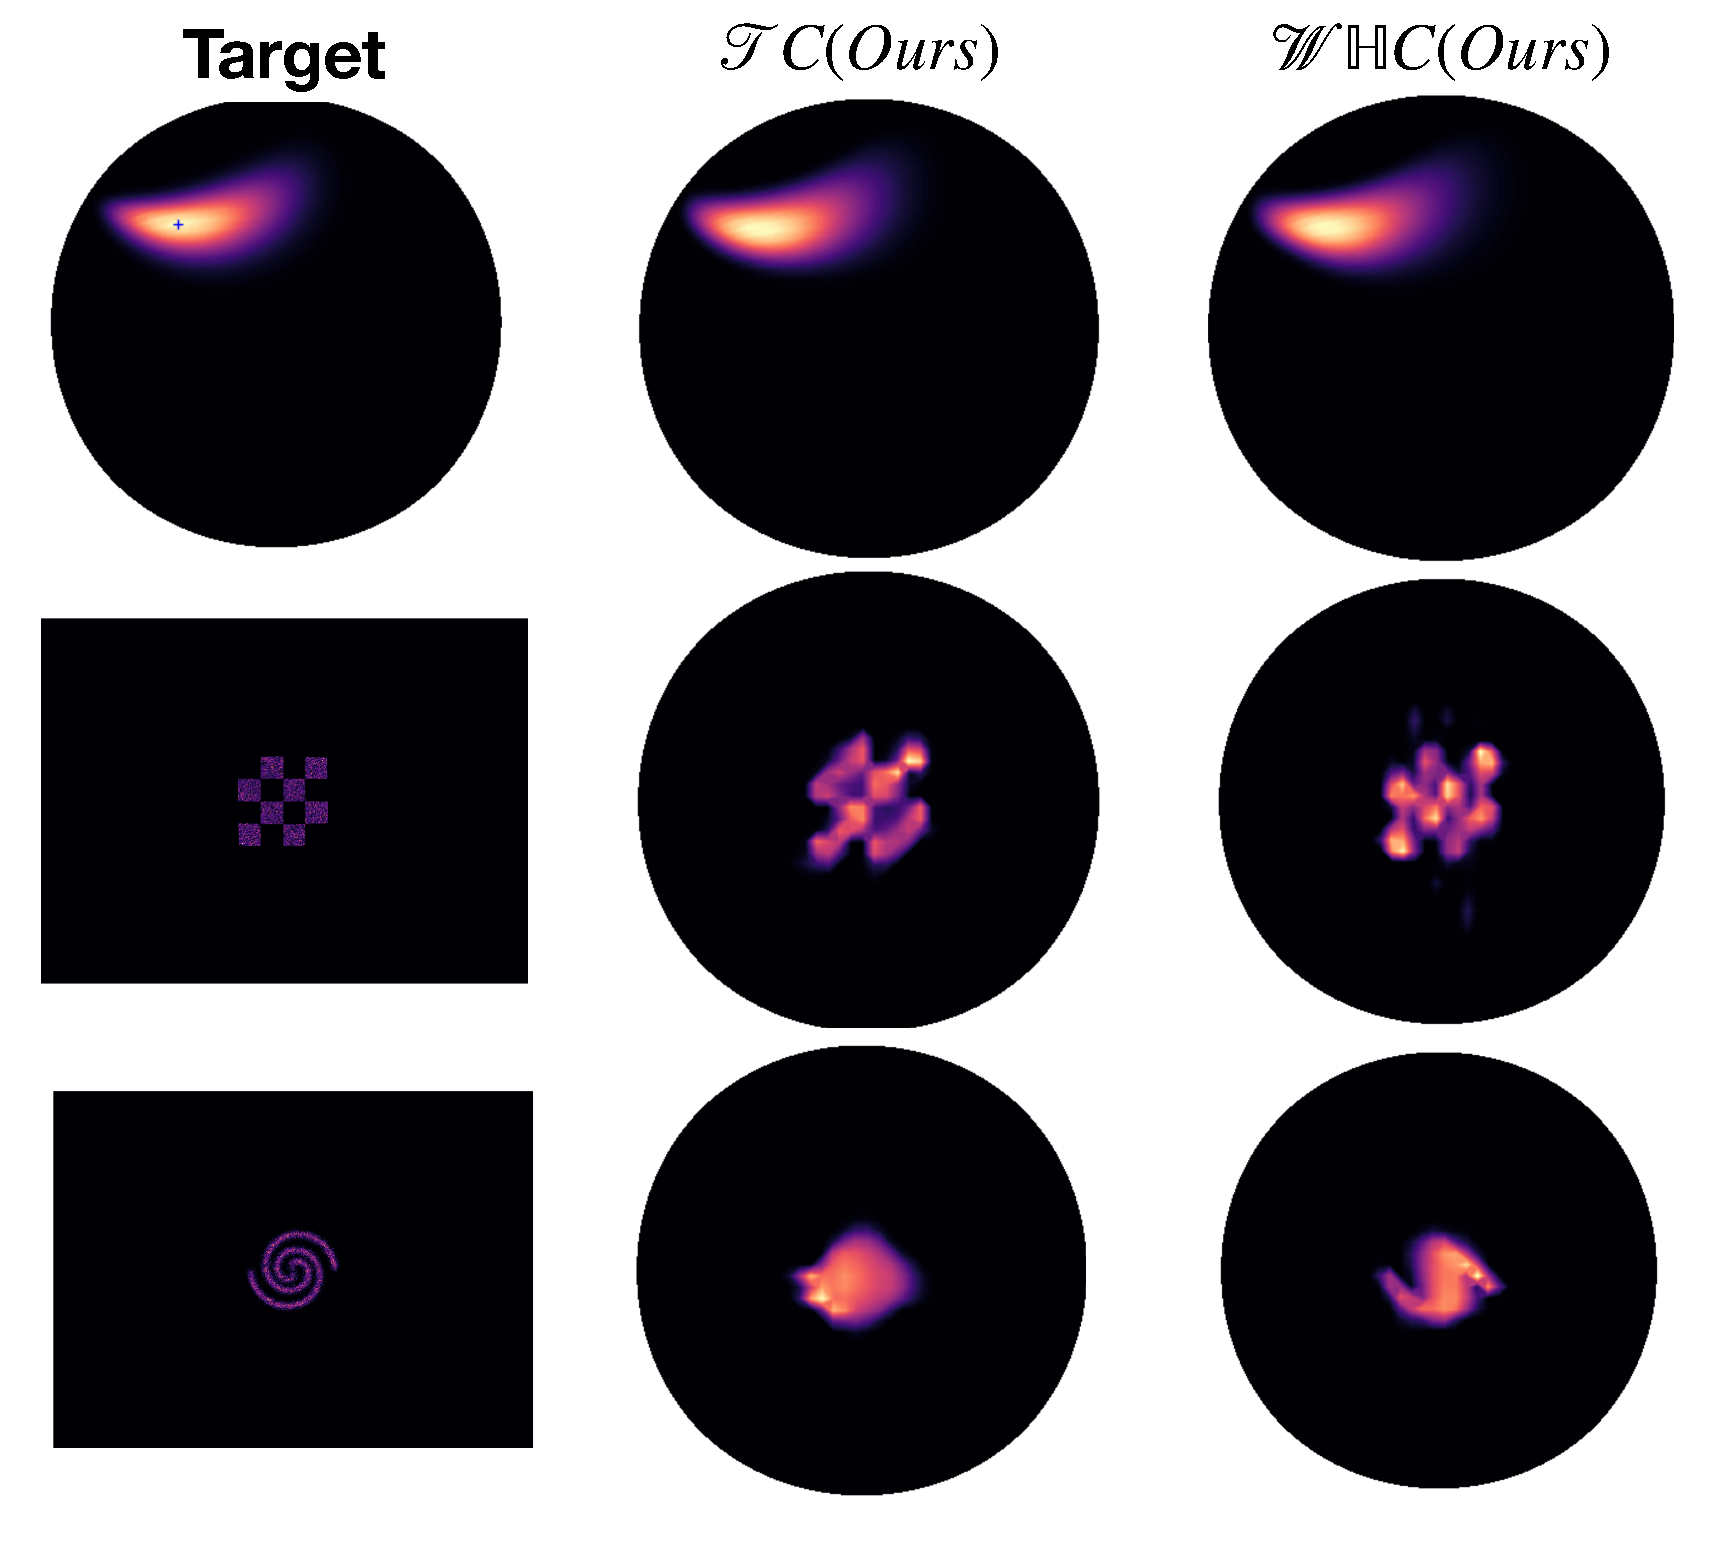
\includegraphics[width=0.95\linewidth]{additional_examples_hyperbolic_density.pdf}
     \caption{\textbf{Top:} Wrapped Gaussian with $\mu = [-1.0,1.0]$ and $\sigma = [1.0, 0.25]^T$. \textbf{Mid:} Checkerboard pattern projected to hyperbolic space. \textbf{Bot:} 2D Spiral projected to hyperbolic space}
     \label{fig:additional_density_estimation}
 \end{figure}
 
 
 
\section{Dataset Issues}
\label{dataset_issues}
Upon inspecting the code and data kindly provided by \citet{mathieu2019continuous} we uncovered some issues that led to us omitting their CS-PhD and Phylogenetics datasets in our comparisons. 
In particular, \citet{mathieu2019continuous} use a decoder in their cross-entropy loss that does not define a proper probability. 
This appears to have caused optimization issues that artificially deflated the reported performance of all the models investigated in that work.
When substituting in the dot product decoder employed in this work, the accuracy of all models increases dramatically. 
After this change, there is no longer any benefit from employing hyperbolic spaces on these datasets. 
In particular, after applying this fix, the performance of the hyperbolic VAE used by \citet{mathieu2019continuous} falls substantially below a Euclidean VAE.
Since we expect our hyperbolic flows to only give gains in cases where hyperbolic spaces provide a benefit over Euclidean spaces, these datasets do not provide a meaningful testbed for our proposed approach. 
Lastly, upon inspecting the code and data in \citet{mathieu2019continuous}, we also found that the columns 1 and 2 in Table 4 of their paper appear to be swapped compared to the results generated by their code. 